\section{Introduction}

Brief introduction to LSST, overview of history of surveys as small-body
discovery machines.

%One of the scientific cornerstones of the Vera C. Rubin Observatory Legacy Survey of Space and Time (LSST)
%is the creation of an unprecedented census of our Solar System.

%\begin{itemize}
%\item LSST Science Requirements Document: \cite{LPM-17}.
%\item LSST overview paper: \cite{2008arXiv0805.2366I}.
%\item LSST Science Book: \cite{abell2009lsst}.
%\end{itemize}

\section{The Vera C. Rubin Observatory and the Legacy Survey of Space and Time}

Half-page summary of key facts about the observatory and the 10-yr survey.

\section{The LSST Solar System Processing Pipeline}

\subsection{Pipeline Design Overview}

High-level overview of pipeline design and key components.

\begin{figure}[th]
\begin{center}
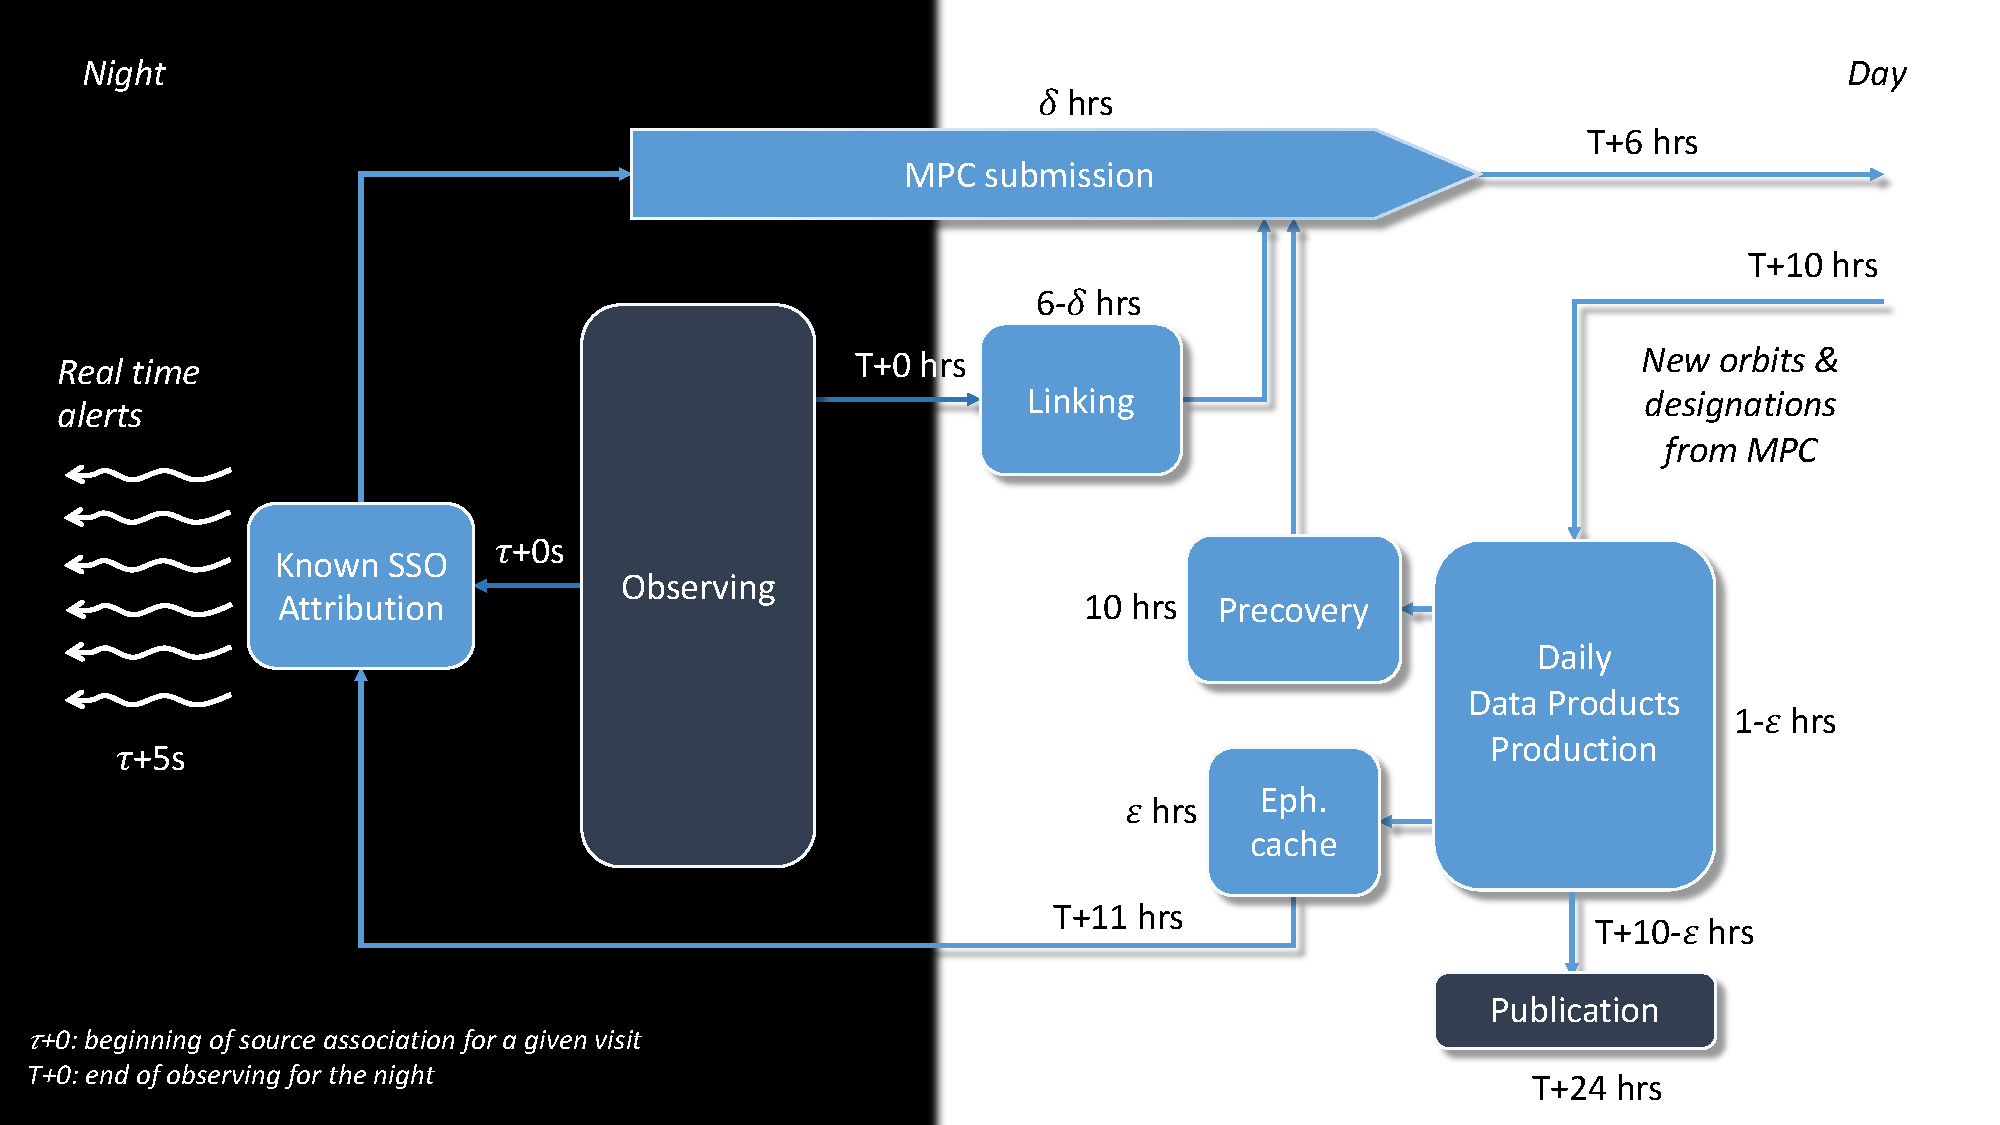
\includegraphics[width=0.9\textwidth]{figures/solarsystempipeline.pdf}

\caption{\label{fig:apMOPS} Detection, attribution, linking, submission and
precovery of moving sources within the nightly data: The attribution is
performed in real-time by the attribution service with resulting information
attached to the alerts and queued for submission to the MPC.  The linking is
performed in daytime, with resulting links queued for submission to the MPC.
Fetching of data from the MPC is performed at least once daily, triggering
recomputation of physical properties and precovery runs.  Any observations
discovered by the precovery procedure are queued for submission to the MPC.
The ephemeris cache is precomputed after the daily fetch of orbit
information from the MPC, to enable fast attribution at nighttime.  All
timings denote design goals.  }

\end{center}
\end{figure}

\subsection{Attribution}
\subsection{Linking}
\subsection{Precovery}
\subsection{Daily Data Product Production}


\section{Data Products}
%\begin{itemize}
%  \item The LSST Data Management System: \cite{2015arXiv151207914J}
%  \item Data Products Definition Document: \cite{LSE-163}
%\end{itemize}

\subsection{Alert Stream Solar System Products}
\subsection{Daily Solar System Data Releases}
\subsection{Yearly Solar System Data Products}

\section{Pipeline Deployment}
\subsection{Solar System Processing during Commissioning}
\subsection{Solar System Processing in the first year of LSST}

\section{Performance Characterization and Validation}

\section{Expected Science Performance for LSST}
\subsection{Expected Discovery Yields}
%LSST Performance for NEO (or moving object) discovery: \cite{2018Icar..303..181J}
\subsection{Characterization Capabilities}
\vspace{0.4cm}


%\begin{itemize}
%\item LSST Catalogs (CatSim): \cite{2014SPIE.9150E..14C}
%\item Feature-Based Scheduler: \cite{2018arXiv181004815N}
%\item Operations Simulator (OpSim): Scheduler \cite{2016SPIE.9910E..13D}, SOCS \cite{2016SPIE.9911E..25R}
%\item Metrics Analysis Framework (MAF): \cite{2014SPIE.9149E..0BJ}
%\item Image simulations (Phosim): \cite{2015ApJS..218...14P}
%\item Sky brightness model: \cite{2016SPIE.9910E..1AY}
%\end{itemize}

\section{Summary}
